%!TEX program=xelatex

% 碰到Windows版本提示Fandol字体,可以在命令行中以管理员权限执行:tlmgr update -self -all
%\documentclass[review]{cvpr}
\documentclass[final]{cvpr}

\usepackage[UTF8]{ctex}

%\usepackage{cvpr}
\usepackage{times}
\usepackage{epsfig}
\usepackage{graphicx}
\usepackage{amsmath}
\usepackage{amssymb}
\usepackage{subfigure}
\usepackage{overpic}


\usepackage{enumitem}
\setenumerate[1]{itemsep=0pt,partopsep=0pt,parsep=\parskip,topsep=5pt}
\setitemize[1]{itemsep=0pt,partopsep=0pt,parsep=\parskip,topsep=5pt}
\setdescription{itemsep=0pt,partopsep=0pt,parsep=\parskip,topsep=5pt}


\usepackage[pagebackref=true,breaklinks=true,colorlinks,bookmarks=false]{hyperref}


%\cvprfinalcopy % *** Uncomment this line for the final submission

\def\cvprPaperID{159} % *** Enter the CVPR Paper ID here
\def\confYear{CVPR 2020}
\def\httilde{\mbox{\tt\raisebox{-.5ex}{\symbol{126}}}}

\newcommand{\cmm}[1]{\textcolor[rgb]{0,0.6,0}{CMM: #1}}
\newcommand{\todo}[1]{{\textcolor{red}{\bf [#1]}}}
\newcommand{\alert}[1]{\textcolor[rgb]{.6,0,0}{#1}}

\newcommand{\IT}{IT\cite{98pami/Itti}}
\newcommand{\MZ}{MZ\cite{03ACMMM/Ma_Contrast-based}}
\newcommand{\GB}{GB\cite{conf/nips/HarelKP06}}
\newcommand{\SR}{SR\cite{07cvpr/hou_SpectralResidual}}
\newcommand{\FT}{FT\cite{09cvpr/Achanta_FTSaliency}}
\newcommand{\CA}{CA\cite{10cvpr/goferman_context}}
\newcommand{\LC}{LC\cite{06acmmm/ZhaiS_spatiotemporal}}
\newcommand{\AC}{AC\cite{08cvs/achanta_salient}}
\newcommand{\HC}{HC-maps }
\newcommand{\RC}{RC-maps }
\newcommand{\Lab}{$L^*a^*b^*$}
\newcommand{\mypara}[1]{\paragraph{#1.}}

\graphicspath{{figures/}}

% Pages are numbered in submission mode, and unnumbered in camera-ready
%\ifcvprfinal\pagestyle{empty}\fi
\setcounter{page}{1}

\begin{document}
% \begin{CJK*}{GBK}{song}

\renewcommand{\figref}[1]{图\ref{#1}}
\renewcommand{\tabref}[1]{表\ref{#1}}
\renewcommand{\equref}[1]{式\ref{#1}}
\renewcommand{\secref}[1]{第\ref{#1}节}
\def\abstract{\centerline{\large\bf 摘要} \vspace*{12pt} \it}

%%%%%%%%% TITLE

\title{网络安全技术期末大作业}

\author{朱浩泽\quad 1911530$^{1}$ \\
    $^{1}$ 南开大学计算机学院
    \\
}

\maketitle
% \thispagestyle{empty}

%%%%%%%%% ABSTRACT
\begin{abstract}
在设计TCP/IP网络协议和OSI标准通信模型的初期,网络设计者关心的问题是如何将数据从一台计算机有效和可拿的传输到另外一台计算机上去。数据的安全性在当时并没有提到议事日程。因此,TCP/IP通信协议和OSI标准通信模型没有内置的安全机制。当人们逐渐意识到这个设计缺陷之后,便想方设法在现有的框架内加入各种安全机制。但是,由于这些通信协议和通信模型不是为网络安全设计的,其体系结构也许并不适用于新的安全功能。为了从根本上纠正这一缺陷,网络设计者们开始研究如下课题:如果从头开始设计网络通信协议,使其包含现有的安全机制及在末来能有效地加入新的安全功能,网络体系结构应该怎样设计才是最好的。本篇文章将在这个问题上进行探讨和研究,包括曾经网络体系结构设计中存在的问题以及如何设计改进一个新的网络体系结构。
\end{abstract}




%%%%%%%%% BODY TEXT %%%%%%%%%%%%%%%%%%%%%%%%%%%%%%%%%%%%%%%%
\section{概述}\label{sec:Introduction}
在最初的网络通信设计过程中,有很多的协议是在大学的课程实验中诞生的。随着时间的推移,这些协议可能在某些特定的应用场景中可以发挥作用,久而久之便成为了某些网络架构的一部分。但是,由于这些网络协议在最初的设计中没有考虑过多的应用场景,而且最初设计网络协议考虑的第一要素一定是是如何将数据从一台计算机有效和可靠的传输到另一台计算机上,所以导致有很多一部分协议是存在着缺陷的,尤其是安全性的问题。

\begin{figure}[t!]
    \begin{overpic}[width=\columnwidth]{SYN.png}
     \end{overpic}
     \caption{TCP的三次握手}
     \label{fig:teaser}
 \end{figure}

近年来,随着科技的高速发展,互联网已经逐渐走入了人们的生活之中,并扮演着不可或缺的作用。在这样的社会背景下,数据安全的重要性愈发展现,网络安全逐渐走进社会,成为了大众关注的一个重点。但是,虽然我们的科技手段愈发的成熟,一些黑客、不法分子等网络破坏者的出现,导致诸如信息泄露等的安全问题频繁发生,这常常给正常的工作生活带来诸多不便或高额的经济损失。而这些问题,常常被归咎于网络协议存在在缺陷,如著名的TCP/IP协议以及OSI标准通信模型在设计的过程中就没有加入安全机制。为了解决这类问题,在此基础之上,根据所学知识,我们将在不改变已经广泛使用的TCP/IP网络协议以及受到广泛认可的OSI标准模型的基础上尝试提出一些简单的、加入了安全机制的网络体系结构的想法。



\section{安全威胁}
TCP/IP协议主要存在的安全问题是IP诈骗,主要包括SYN洪水攻击、TCP劫持、ARP诈骗和IP碎片攻击等。

\paragraph*{SYN洪水攻击} 在TCP/IP协议中,两台客户端之间如果要进行通讯,朔县需要进行三次握手,如图\ref*{fig:teaser},服务端的资源分配时在第二次握手时分配的,而客户端资源时在完成第三次握手时分配的。所以服务端容易收到SYN泛洪攻击,其具体形式为攻击目标主机的TCP缓冲区,攻击者向攻击目标发送大量SYN请求,利用TCP/IP网络协议中产生的副作用,用SYN控制包占满对方缓冲区,使得被攻击的计算机不能与其他计算机建立通信。
\paragraph*{TCP劫持} 攻击者用网络嗅探软件截获建立TCP连接的SYN控制包,根据其中的信息伪造回应控制包,从而以被攻击者的名义与服务器建立连接。
\paragraph*{IP碎片攻击} 由于IP协议无法检测源IP的合法性与真实性,攻击者可以向被攻击者发送大量的IP分片,被攻击者在收到这些大量的IP分片后,会对IP分片进行重组,重组大量的IP分片将大量占用被攻击者的计算资源,攻击严重的情况下,很可能会使得被攻击者陷入系统雍疾。
\paragraph*{ARP诈骗} 受害者主机的IP地址的相应MAC地址被偷换成攻击者选择的MAC地址,攻击者以此取代受害者与他人通信。
\\ 

除此之外,网络中还有着一些不安全的其他因素,如通过IP包进行流量分析、Dos攻击、DNS劫持等攻击手段或设计缺陷。





% 人类可以很容易地判断图像中的显著性区域,并注意到图像的重要部分。
% 由于我们可以通过显著性区域来优先分配图像分析与合成所需的计算资源,
% 所以通过计算来检测图像的显著性区域意义重大。
% 提取出的显著性图像可以广泛应用于许多计算机视觉领域的应用,
% 包括对兴趣目标物体图像分割~\cite{06TCSVT/han_unsupervised,06josa/KoN_InterestSegmentation},
% 目标识别~\cite{04cvpr/RutishauserWWKP},自适应压缩~\cite{00CE/christopoulos_jpeg},
% 内容感知图像编辑~\cite{TOG/Wang08,09cgf/ZhangC,wu-2010-resizing,10vc/Ding},
% 和图像检索~\cite{tog09/ChenCT_Sketch2Photo}等。


% \begin{figure}[t!]
%    \begin{overpic}[width=\columnwidth]{teaser.pdf}
%     \end{overpic}
%     \caption{给定输入图像(上),可以通过全局对比度分析得到高分辨率的视觉显著性图(中)。
%          这种视觉显著性图可以进一步被用来获取感兴趣物体区域(下)。
%     }\label{fig:teaser}
% \end{figure}


% \begin{figure*}[t!]
%    \begin{overpic}[width=\textwidth]{all_comparisons.pdf} \small
%    \put(0.3,0){(a)~输入图}
%    \put(10,0){(b)~\IT}
%    \put(18.3,0){(c)~\MZ}
%    \put(27.5,0){(d)~\GB}
%    \put(37,0){(e)~\SR}
%    \put(46.5,0){(f)~\AC}
%    \put(55.5,0){(g)~\CA}
%    \put(65,0){(h)~\FT}
%    \put(73.5,0){(i)~\LC}
%    \put(84,0){(j)~HC}
%    \put(93,0){(k)~RC}
%    \end{overpic}
%    \caption{通过现有最先进的一组方法(b-i),以及我们提出的HC方法(j)和RC方法(k)
%       得到的视觉显著性图。其中的许多方法更加强调边或者只能得到低分辨率的显著性图。
%       \figref{fig:VisualComparison}和我们的项目主页中有更多的结果。
%    }\label{fig:cmp1vAll}
% \end{figure*}


% 显著性源于视觉的独特性、不可预测性、稀缺性以及奇异性,并且是由颜色、梯度、边缘、
% 边界等图像属性所致。
% 视觉显著性和我们如何感知、处理视觉刺激紧密相关,
% 并且正在被包括认知心理学~\cite{55ARP/Teuber_physiological,04nature/Wolfe_attributesVisual},
% 神经生物学~\cite{95ARN/DesimoneNeuralMachanisms,09biology/eyeMovement}
% 和计算机视觉~\cite{98pami/Itti,09cvpr/Achanta_FTSaliency}在内的多个学科进行研究。
% 关于人类视觉注意的理论假设人类视觉系统只详细地处理图像的某个局部,而不是整幅图像。
% Treisman 和 Gelade~\cite{80cogSc/Treisman_featureIntegration}, Koch 和
% Ullman~\cite{85HN/KochVisualAttention}的早期工作,以及Itti, Wolfe 等人的视觉注意理论提议将视觉注意机制分为两个阶段:
% 快速的、下意识的、自底向上的、数据驱动的显著性提取;
% 以及慢速的、任务依赖的、自顶向下的、目标驱动的显著性提取。


% 我们依据图像的对比度来进行自底向上、数据驱动的显著性检测。
% 人们普遍认为,为了优先响应高对比度刺激,人类的大脑皮质细胞在它们
% 的接受域可能是\emph{硬编码}的~\cite{03neuron/Reynolds_attentionSaliency}。
% 基于以下观察,我们提出了提取高分辨率的全局显著性图像的分析方法:
% \begin{itemize}
%     \item 基于全局对比度的方法倾向于将大范围的目标和周围环境分离开。
%         这种方法要优于那些通常只在轮廓附近产生较高显著性的局部对比度方法。
%     \item 全局的考虑可以为图像中相似区域分配一个相近的显著性的值,并且可以均匀的突出目标。
%     \item 一个区域的显著性,主要是由它和周围区域的对比度决定,相距很远的区域起的作用较小。
%     \item 为了能够适应大规模图像集处理和高效的图像检索与分类的应用需求,
%         显著图检测算法应该具有简单快速的特点。
% \end{itemize}


% 我们提出了\emph{基于直方图对比度的方法}~(HC) 来检测显著性。
% \HC 依据与其它像素的色彩差异来分配像素的显著性值,并用以产生具有全分辨率显著性图像。
% 我们用基于直方图的方法来进行高效处理,并用色彩空间的平滑操作来控制量化的缺陷。
% 我们的算法致力于处理普通的自然景象,对处理具有高纹理的图像场景不一定能达到最佳效果
% (见 \figref{fig:challenging_maps})。


% 作为HC-map的改进,我们结合空间关系来获取\RC 。首先将图像分割成区域,
% 再为每个区域分配显著性值,从而形成\emph{基于局域对比度的}~(RC)显著性图。
% 区域的显著性值由全局对比度值计算得到。
% 这种全局对比度值由当前区域相对于其它区域的对比度以空间距离来度量。


% 我们在国际上现有最大的公开基准数据集上广泛地测试了我们的结果,
% 并且与现有最先进的一组显著性图像提取方法
% ~\cite{98pami/Itti,03ACMMM/Ma_Contrast-based,06acmmm/ZhaiS_spatiotemporal,conf/nips/HarelKP06,07cvpr/hou_SpectralResidual,08cvs/achanta_salient,09cvpr/Achanta_FTSaliency,10cvpr/goferman_context}
% 的结果,以及人工标注的参考数据进行了比较
% \footnote{对1000幅测试图得到的结果以及软件原型可以从我们的项目主页上获取:
% \href{http://cg.cs.tsinghua.edu.cn/people/~cmm/saliency/}
% {http://cg.cs.tsinghua.edu.cn/people/\%7Ecmm/saliency/}}.
% 我们的方法和之前已有的方法相比,在正确率和召回率方面都有明显的提高。
% 总地来说,和 HC-map相比比, RC-map的正确率和召回率更高,但是计算量也更高。
% 令人欣慰的是,利用我们的显著性图像分割出来的区域在大多数情况下符合人工的标注。
% 我们还将提取出的显著性图像应用于图像分割,内容感知的图像缩放,以及非真实感渲染等应用。


%%%%%%%%%%%%%%%%%%%%%%%%%%%%%%%%%%%%%%%%%%%%%%%%%%%%%%%%%%%%%%%%%%%%%%%%%%%%%%%%%
\section{相关工作}
\label{sec:RelatedWorks}

本文主要关注自底向上的显著性检测相关的相关文献。
这类方法或是基于生物学原理的,或是纯计算的,或两者兼顾。
这些方法利用亮度、颜色、边缘~\cite{09cvpr/Achanta_FTSaliency}
等底层特征属性来决定图像某个区域和它周围的对比度。
我们宽泛地把这些算法分类为局部的和全局的两大类。

基于局部对比度的方法利用图像区域相对于局部邻域的稀有度。
在Koch和Ullman~\cite{85HN/KochVisualAttention}提出的非常有影响力的生物启发模型基础上,
Itti等人~\cite{98pami/Itti}定义了图像的显著性。
此定义利用了多尺度图像特征的中心-周围的差异来得到。
Ma和Zhang~\cite{03ACMMM/Ma_Contrast-based}
提出了另一种局部对比度分析方法来产生显著性图像,并用模糊增长模型对其进行扩展。
Harel等人~\cite{conf/nips/HarelKP06}通过将Itti等人的特征图归一化来突出显著部分,
并且可以和其它显著图像结合。
Liu等人~\cite{10pami/Liu_Learning}通过将高斯图像金字塔的对比度线性结合,
提出了多尺度对比度。
最近,Goferman等人~\cite{10cvpr/goferman_context}
同时对局部底层线索、全局考虑、视觉组织规则以及表层特征进行建模来突出显著性物体。
这些利用局部对比度的方法倾向于在边缘部分产生高显著性值,
而不是均匀地突出整个物体(见\figref{fig:cmp1vAll})。

基于全局对比度的显著性区域计算方法用一个区域和整个图像的对比度来计算显著性值。
Zhai和Shah~\cite{06acmmm/ZhaiS_spatiotemporal}定义了基于某个像素和其余像素点
对比度的像素级显著性。
Achanta 等人~\cite{09cvpr/Achanta_FTSaliency}提出了频率调谐方法,
此方法用某个像素和整个图像的平均色的色差来直接定义显著性值。
但它该方法只考虑了一阶平均颜色,不足以分析复杂多变的自然图像。
图~\ref{fig:VisualComparison}和图~\ref{fig:plots}展示了这种方法定性和定量的缺点。
此外,这些方法忽略了图像各部分间的空间关系,
而这个因素对可靠的显著性检测来说可能是至关重要的(见\secref{sec:Experiment})。


%%%%%%%%%%%%%%%%%%%%%%%%%%%%%%%%%%%%%%%%%%%%%%%%%%%%%%%%%%
\section{基于直方图统计的对比度}\label{sec:HC}

生物视觉研究关于视觉显著性的观察认为,视觉系统对视觉信号的对比度是很敏感的。
据此,我们基于输入图像的颜色统计特征提出了基于直方图对比度
(Histogram Contrast, HC)的图像像素显著性值检测方法。
具体来说,一个像素的显著性值用它和图像中其它像素颜色的对比度来定义。
例如,图像$I$中像素$I_k$的显著性值定义为:
\begin{equation}\label{equ:PixelColorContrast}
    S(I_k) = \sum_{\forall I_i \in I} D(I_k, I_i),
\end{equation}
其中 $D(I_k, I_i)$ 为 像素$I_k$ 和像素$I_i$ 在\Lab 空间的颜色距离度量
(参考~\cite{06acmmm/ZhaiS_spatiotemporal})。
\equref{equ:PixelColorContrast} 可以按照像素顺序展开为以下形式:
\begin{equation}\label{equ:PixelCCPixelOrder}
    S(I_k) = D(I_k, I_1) + D(I_k, I_2) + \cdots + D(I_k, I_N),
\end{equation}
其中 $N$ 为图像 $I$ 的像素数。
我们可以看到,由于忽略了空间关系,在这种定义下具有相同颜色值得像素具有相同的显著性值。
因此我们可以对\equref{equ:PixelCCPixelOrder}进行重排,
使得具有相同颜色值$c_j$的像素归到一起,得到每个颜色的显著性值:
\begin{equation}\label{equ:PixelCCColorOrder}
    S(I_k) = S(c_l) = \sum_{j=1}^{n}{f_j D(c_l, c_j)},
\end{equation}
其中$c_l$ 为像素$I_k$的颜色值,$n$为图像中所含的颜色总数,
$f_j$为$c_j$在图像$I$中出现的概率。

%%%%%%%%%%%%%%%%%%%%%%%%%%%%%%%%%%%%%%%%%%%%%%%

\mypara{基于直方图的加速}用\equref{equ:PixelColorContrast}
来朴素地计算图像每个像素显著性值的方法的时间复杂度为$O(N^2)$。
对于中等图像来说,计算代价已经非常高了。
上述公式的等价表示\equref{equ:PixelCCColorOrder}花费$O(N) + O(n^2)$ 的时间。
如果 $O(n^2) \leq O(N)$,时间复杂度可以改进到$O(N)$。
因此,加速的关键在于减少图像像素颜色的总数。
然而,真彩色空间包含$256^3$种可能的颜色,比图像的像素总数多很多。

Zhai和Shah~\cite{06acmmm/ZhaiS_spatiotemporal}仅仅用了亮度来减少颜色的数量 $n$。
这种方法得到的$n^2=256^2$($256^2 \ll N$)。
然而,他们的方法的缺陷在于忽略了颜色信息的可区别性。


\begin{figure}
  	\begin{overpic}[width=\columnwidth]{histogram.pdf}
    \end{overpic}
    \caption{给定一个输入图像(左),我们计算其颜色直方图(中)。
        直方图中每一个bin所对应的颜色在下方的横条中显示。
        量化后的图像仅仅使用$43$个直方图bin的色彩,
        且仍然保留了显著性检测所需的足够的视觉质量。
    }\label{fig:colorFre}
\end{figure}


在这个的工作中,我们用全色彩空间来代替仅用亮度的方法。
为了减少需要考虑的颜色数目,我们先将每个通道的颜色量化得到12个不同的值,
这会将颜色数量减少到$12^3=1728$。
考虑到自然图像中的颜色只占据整个色彩空间很小的一部分,
我们可以将出现频率较小的颜色丢掉以减少色彩数目。
通过选择高频出现的颜色,并确保这些颜色覆盖$95\%$以上的像素,
我们可以做到将颜色数目减少到$n=85$左右(实验结果详见\secref{sec:Experiment} )。
剩下的小于$5\%$的像素所占的颜色被直方图中距离最近的颜色所代替。
\figref{fig:colorFre}为典型的量化样例。
请再次注意,基于时间性能的考虑,
我们用简单的基于直方图的量化方法来代替优化一幅图像的特定颜色。


%%%%%%%%%%%%%%%%%%%%%%%%%%%%%%%%%%%%%%%%%%%%%%


\mypara{颜色空间平滑}
虽然我们可以用颜色量化后的颜色直方图来高效计算颜色对比度,但量化本身可能会产生瑕疵。
因为一些相似的颜色可能被量化为不同的值。
为了减少这种随机性给显著性值计算带来的噪声,我们用平滑操作来改善每个颜色的显著性值。
每个颜色的显著性值被替换为相似颜色(用\Lab 距离测量)显著性值的加权平均。
这个过程实质上是颜色空间的一种平滑过程。
我们选择$m=n/4$个最近邻颜色来改善颜色$c$的显著性值,见公式:
\begin{equation}\label{equ:smoothing}
    S'(c) = \frac{1}{(m-1)T} \sum_{i=1}^{m} (T-D(c, c_i))S(c_i)
\end{equation}
其中 $T=\sum_{i=1}^{m} D(c, c_i)$ 为颜色 $c$和它的$m$ 个最近邻$c_i$之间的距离,
归一化因数由以下公式得到:
\begin{equation*}\label{equ:smoothingN}
    \sum_{i=1}^{m} (T-D(c, c_i))=(m-1)T.
\end{equation*}
我们用了一个线性变化平滑权值$(T-D(c, c_i))$来为在颜色特征空间中距离
$c$ 较近的颜色分配较大权值。
在我们的实验中,我们发现这种线性变化的权值比急剧下降的高斯权值的效果好。
\figref{fig:HCSmoothing}为颜色空间平滑后的效果,按显著性值降序排列。
注意到相似的直方图区间在平滑过后会非常接近,表明相似的颜色非常可能分配到相似的显著性值,
因此减少了量化的瑕疵(见 \figref{fig:plots})。


\mypara{实现细节}
为了将颜色空间量化为$12^3$种不同的颜色,我们统一将每个颜色的通道划分为12个等级。
虽然颜色量化在 RGB 颜色空间进行,
但为了颜色距离计算与人类感知更加符合,我们在 \Lab 颜色空间来测量颜色的距离。
我们并不直接在\Lab 颜色空间进行量化,因为并不是所有在区间$L^*\in[0, 100]$,
$a^*, b^*\in[-127,127]$中的颜色都对应真实的颜色。
实验结果表明,直接在 \Lab 空间量化得到效果并不好。
最佳结果是在 RGB 颜色空间量化,在\Lab 颜色空间测量距离得到的。


\begin{figure}[t]
    \centering
    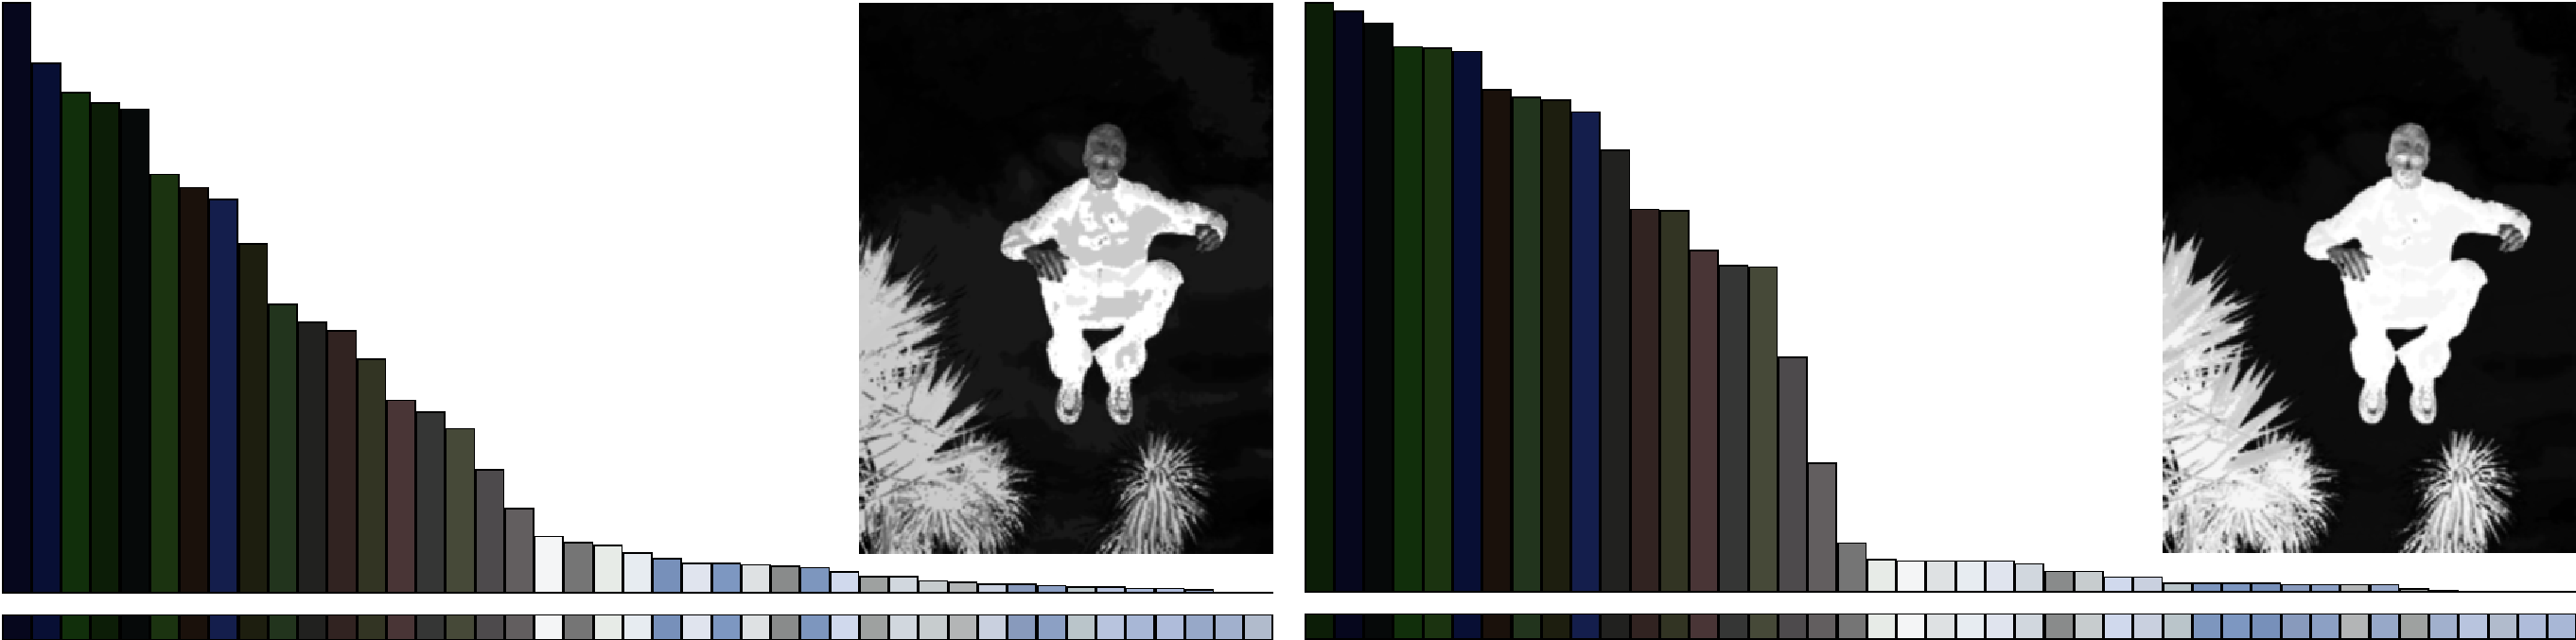
\includegraphics[width=\columnwidth]{histogram_saliency.pdf}
    \caption{颜色空间平滑前(左)后(右)像素颜色的显著性值
        (归一化到$[0, 1]$)。
        对应的显著性图在各自的内嵌插图中显示。
    }\label{fig:HCSmoothing}
\end{figure}

%%%%%%%%%%%%%%%%%%%%%%%%%%%%%%%%%%%%%%%%%%%%%%%%%%%%%%%%%%
\section{基于区域的对比度}

\begin{figure}[b]
    \centering
    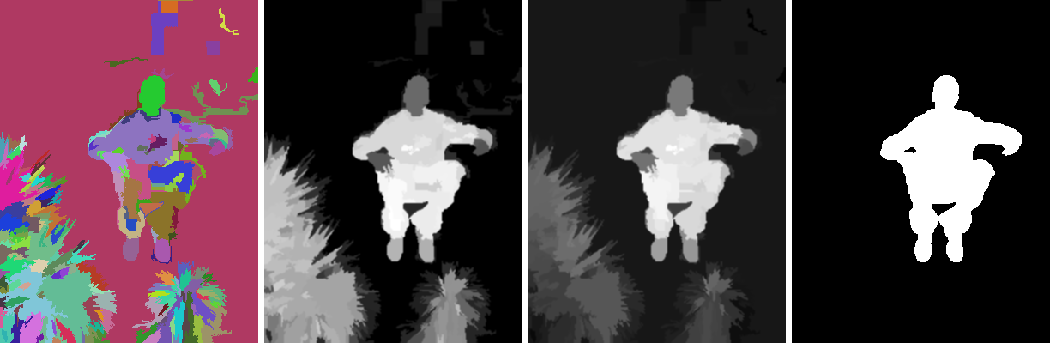
\includegraphics[width=\columnwidth]{region_contrast.pdf}\\
    \caption{由Felzenszwalb和Huttenlocher的分割方法
        \cite{04ijcv/felzenszwalb_efficient}得到的图像区域(左),
        考虑(中-右)和不考虑(中-左)距离权值分别得到的区域对比度。
        通过考虑空间关系,我们得到的高质量的重要性分割结果(右)可以和人工分割结果相比。
    }\label{fig:regContrast}
\end{figure}


\begin{figure*}[t]
   \begin{overpic}[width=\textwidth]{comparison.pdf} \small
   \put(3,0){(a)~original}
   \put(18.5,0){(b)~LC}
   \put(33,0){(c)~CA}
   \put(48,0){(d)~FT}
   \put(60,0){(e)~\HC}
   \put(74,0){(f)~\RC}
   \put(90,0){(g)~RCC}
   \end{overpic}
   \caption{显著性图的视觉效果对比。(a)原图,由以下方法产生的显著性图
       (b) Zhai和Shah\cite{06acmmm/ZhaiS_spatiotemporal},
       (c) Goferman等\cite{10cvpr/goferman_context},
       (d) Achanta等\cite{09cvpr/Achanta_FTSaliency},
       (e) 我们的HC和(f)RC方法,和(g)基于RC图的显著性区域分割结果.
       我们的方法的结果均匀的突出整个显著性区域。
       整个数据集上的所有检测结果可以从我们的项目主页上获取。
   }\label{fig:VisualComparison}
\end{figure*}


人们会更加注意到图像中和周围物体对比度非常大的区域
\cite{03neuroscience/luminanceContrast}。
除了对比度之外,空间关系在人类注意力方面也起到非常大的作用。
相邻区域的高对比度比很远区域的高对比度更容易导致一个区域引起视觉注意。
在计算像素级对比度时引进空间关系计算代价会非常大,
我们引进一种对比度分析方法:\emph{区域对比度} (Region Contrast, RC),
以此来将空间关系和区域级对比度计算结合到一起。
在RC方法中,我们首先将图像分割成若干区域,
然后计算区域及颜色对比度,再用每个区域和其它区域对比度加权和来为此区域定义显著性值。
权值由区域空间距离决定,较远的区域分配较小的权值。


%%%%%%%%%%%%%%%%%%%%%%%%%%%%%%%%%%%%%%%%%%%%%%%%%%%%%%%%%%
\mypara{用稀疏直方图比较来计算区域对比度}
首先,我们用基于图的图像分割方法将输入图像分割成若干区域
\cite{04ijcv/felzenszwalb_efficient}。
然后为每个区域建立颜色直方图\secref{sec:HC}。
对每个区域$r_k$,我们通过测量它与图像其它区域的颜色对比度来计算它的显著性值,
\begin{equation}\label{equ:regContrastSaliency}
    S(r_k) = \sum_{r_k \neq r_i} w(r_i)  D_r(r_k, r_i),
\end{equation}
其中$w(r_i)$为区域$r_i$的权值,$D_r(\cdot, \cdot)$为两个区域的颜色距离度量。
这里我们用 $r_i$里的像素数$w(r_i)$ 来强调大区域的颜色对比度。
两个区域$r_1$和$r_2$的颜色距离为:
\begin{equation}\label{equ:regContrast}
    D_r(r_1, r_2) = \sum_{i=1}^{n_1} \sum_{j=1}^{n_2} f(c_{1,i}) f(c_{2,j}) D(c_{1,i}, c_{2,j})
\end{equation}
其中$f(c_{k,i})$为第$i$个颜色$c_{k,i}$在第$k$个区域$r_k$的所有$n_k$种颜色中
出现的概率,$k=\{1,2\}$。
注意到我们使用区域的概率密度函数(即归一化的颜色直方图)中颜色出现概率作为权值,
以强调主要的颜色之间的区别。

因为每个区域只包含图像的直方图中很少数目的颜色,
所以为每个区域存储和计算常规矩阵形式的直方图是低效的。
我们用稀疏直方图以使得存储和计算过程更加高效。


%%%%%%%%%%%%%%%%%%%%%%%%%%%%%%%%%%%%%%%%%%%%%%%%%%%%%%%%%%

\begin{table*}
    \centering
    \begin{tabular}{l|c|c|c|c|c|c|c|c|c|c} \hline\hline
      方法  &  \IT   &  \MZ  &   \GB  &  \SR   &  \FT  &  \AC  &  \CA   & \LC   &  HC   &  RC   \\ \hline
      时间(秒) & 0.611  & 0.070 & 1.614  & 0.064  & 0.016 & 0.109 &  53.1  & 0.018 & 0.019 & 0.253 \\ \hline
      代码类型    & Matlab & C++   & Matlab & Matlab &  C++  &  C++  & Matlab &  C++  &  C++  &  C++  \\ \hline\hline
    \end{tabular}
    \caption{计算Achanta等人数据集\cite{09cvpr/Achanta_FTSaliency}中图像的平均用时。
        该数据集(参见我们主页)中大部分的图像分辨率为$400\times300$。
        这里所示的所有方法的时间是在一个拥有Dual Core 2.6 GHz
        CPU,2GB内存的机器上测得的。
    } \label{tab:TimeEfficency}
\end{table*}


\mypara{空间加权区域对比度 }
更进一步,通过在\equref{equ:regContrastSaliency}中引进空间权值,
我们将空间信息加入进来,来增加区域的空间影响效果。
近邻的区域增大影响,较远的区域减小影响。
特别地,对任意区域 $r_k$,基于空间加权区域对比度的显著性定义为:
\begin{equation}\label{equ:regContrastSpatial}
    S(r_k)=\sum_{r_k\neq r_i}\exp({-D_s(r_k,r_i)/\sigma_s^2})w(r_i) D_r(r_k, r_i)
\end{equation}
其中 $D_s(r_k, r_i)$ 为区域$r_k$ 和 $r_i$的空间距离,$\sigma_s$控制空间权值强度。
$\sigma_s$ 越大,空间权值的影响越小,导致较远区域的对比度会对当前区域显著性值做出较大的贡献。
两个区域的空间距离定义为两个区域重心的欧氏距离。在我们的试验中,$\sigma_s^2 = 0.4$,像素坐标归一化到$[0, 1]$区间。


%%%%%%%%%%%%%%%%%%%%%%%%%%%%%%%%%%%%%%%%%%%%%%%%%%%%%%%%%%%%%%%%%%%%%%
\section{实验比较}\label{sec:Experiment}


我们在Achanta等人提供的公开测试集\cite{09cvpr/Achanta_FTSaliency}上测试了我们的方法。
据我们所知,此测试集是此类数据最大的测试集,并且由人工精确标注了显著性区域。
我们将基于全局对比度的方法与其它$8$个当今最好的方法进行了比较。
仿照\cite{09cvpr/Achanta_FTSaliency},我们依据以下几个方面来选择其它方法来进行对比:
引用数(\IT ~和 \SR)、较新的方法(\GB, SR, \AC, \FT ~and \CA)、
多种类(IT 为生物驱动, \MZ~为纯计算, GB 为两者混合的, SR 在频域进行处理,
AC and FT 输出全分辨率显著性图),和我们方法最接近的(\LC)。


我们的方法和其它的方法在1000张图片上计算得到了显著性图。
\tabref{tab:TimeEfficency} 比较了每个方法的平均用时。
我们的方法HC和RC用C++实现,对于IT、GB、SR、FT和CA,我们引用了作者的实现。
由于找不到LC作者的源码,我们用C++来实现了此算法。
对于典型自然图片,HC 方法时间复杂度为 $O(N)$,对于实时应用已经非常高效。
相比之下,RC需要图像分割~\cite{04ijcv/felzenszwalb_efficient},
所以较慢,但它产生更好的效果。

\begin{figure*}[t]
  \centering
  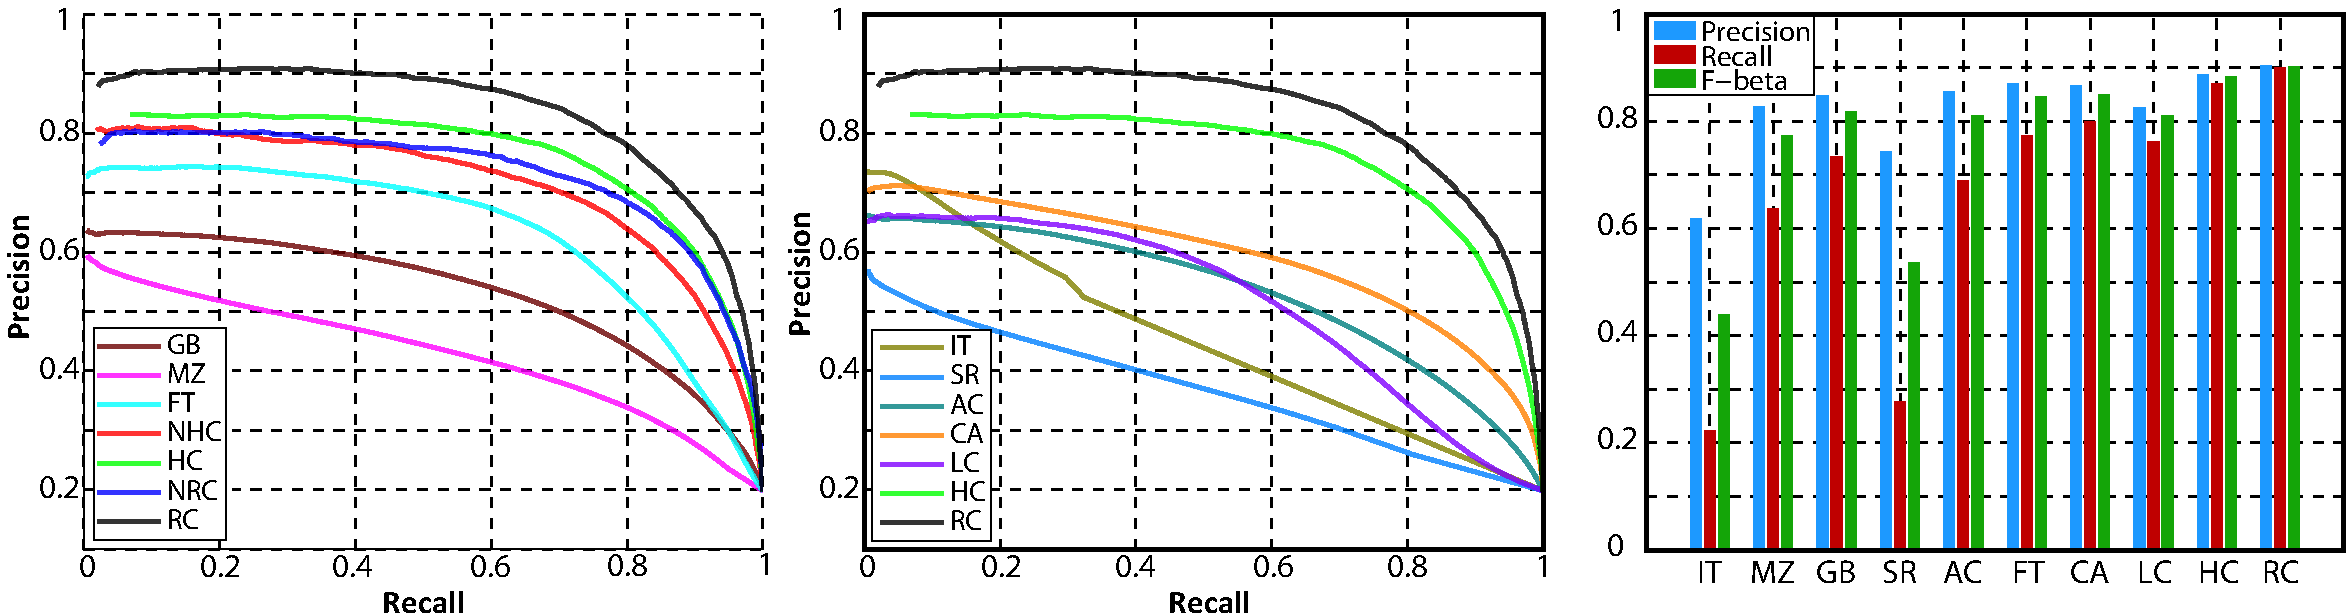
\includegraphics[width=\textwidth]{plots.pdf}
  \caption{在包含1000副图像的公开测试集上各种方法检测得到的显著性图经过
      简单阈值分割得到结果的正确率召回率曲线。
      左图和中图是我们方法不同配置与\GB, \MZ,  \FT, \IT, \SR, \AC, \CA,和\LC
      等方法的比较。
      NHC代表我们HC方法不带颜色空间平滑,NRC代表我们RC方法不带空间加权。
      右图是我们显著性区域分割方法以不同的显著性图作为初始值得到的正确率召回率柱状图。
      我们的RC方法在1000副图像数据集上的结果具高的精度,召回率和$F_{\beta}$值。
      (相关的结果图像从我们的项目主页上可以得到。)
  } \label{fig:plots}
\end{figure*}

为了全面的测试我们提出的方法的准确性,我们用了两种不同的客观比较方法进行了试验。
在第一个实验中,为了分割显著性物体并计算准确率召回率曲线,
我们参考\cite{09cvpr/Achanta_FTSaliency},用所有阈值分别将显著性图进行二值化。
在第二个试验中,我们用显著性图像初始化后迭代应用GrabCut方法
\cite{04tog/rother_grabcut}进行显著性物体分割。
我们还将得到的显著性图作为内容敏感的图像缩放和非真实感渲染的重要性权值。


%%%%%%%%%%%%%%%%%%%%%%%%%%%%%%%%%%%%%%%%%%%%%%%%%%%%%%%%%

\mypara{固定阈值的分割}
得到显著性物体的二值分割的最简单方法就是设定一个$T_f \in [0, 255]$的阈值。
为了可靠地比较多样的显著性检测方法高亮显著性物体的效果,
我们将阈值$T_f$设定为在$0$到$255$之间变化。\figref{fig:plots}为精确度召回率曲线结果。
我们还介绍了加入色彩空间平滑以及空间权值后的效果以及与其它方法的比较。
这些方法得到的显著性图的视觉直观比较在图~\ref{fig:cmp1vAll}
和图\ref{fig:VisualComparison}中。

正确率、召回率曲线清楚地展示出我们的方法优于其它的八种方法。
曲线的极限很有趣:在$T_f=0$处召回值最大,所有的像素被认为是前景,
所以所有的方法得到相同的正确值和召回值;这点的正确值为$0.2$,召回值为$1.0$。
这表明,在标注数据中,平均$20\%$的图像像素属于显著性区域。
曲线另一端,我们的方法的最小召回值比其它方法高,
因为我们的显著性图更加平滑,且包含更多显著性值为$255$的像素。


%%%%%%%%%%%%%%%%%%%%%%%%%%%%%%%%%%%%%%%%%%%%%
\mypara{显著性分割}
我们考虑将计算所得的显著性图像用于帮助显著物体分割。
在已有的工作中,显著性图已经被用于非监督物体分割:Ma和Zhang\cite{03ACMMM/Ma_Contrast-based}
通过在显著性图上进行模糊区域增长来找到矩形显著的区域。
Ko和Nam\cite{06josa/KoN_InterestSegmentation}在图像线段特征上训练支持向量机,
然后将这些区域聚类来提取显著性物体。
Han等人\cite{06TCSVT/han_unsupervised}用颜色、纹理和边缘特征建立马尔可夫
随机场模型,用显著性图的种子值来增长显著性物体区域。
最近,Achanta 等人~\cite{09cvpr/Achanta_FTSaliency}先通过mean-shift分割得到图像区域,
然后再图像区域内对显著性值进行平均,
再通过识别平均显著性值大于整个图像平均显著性值的2倍的图像区域来确定显著性区域。

\begin{figure}[b]
    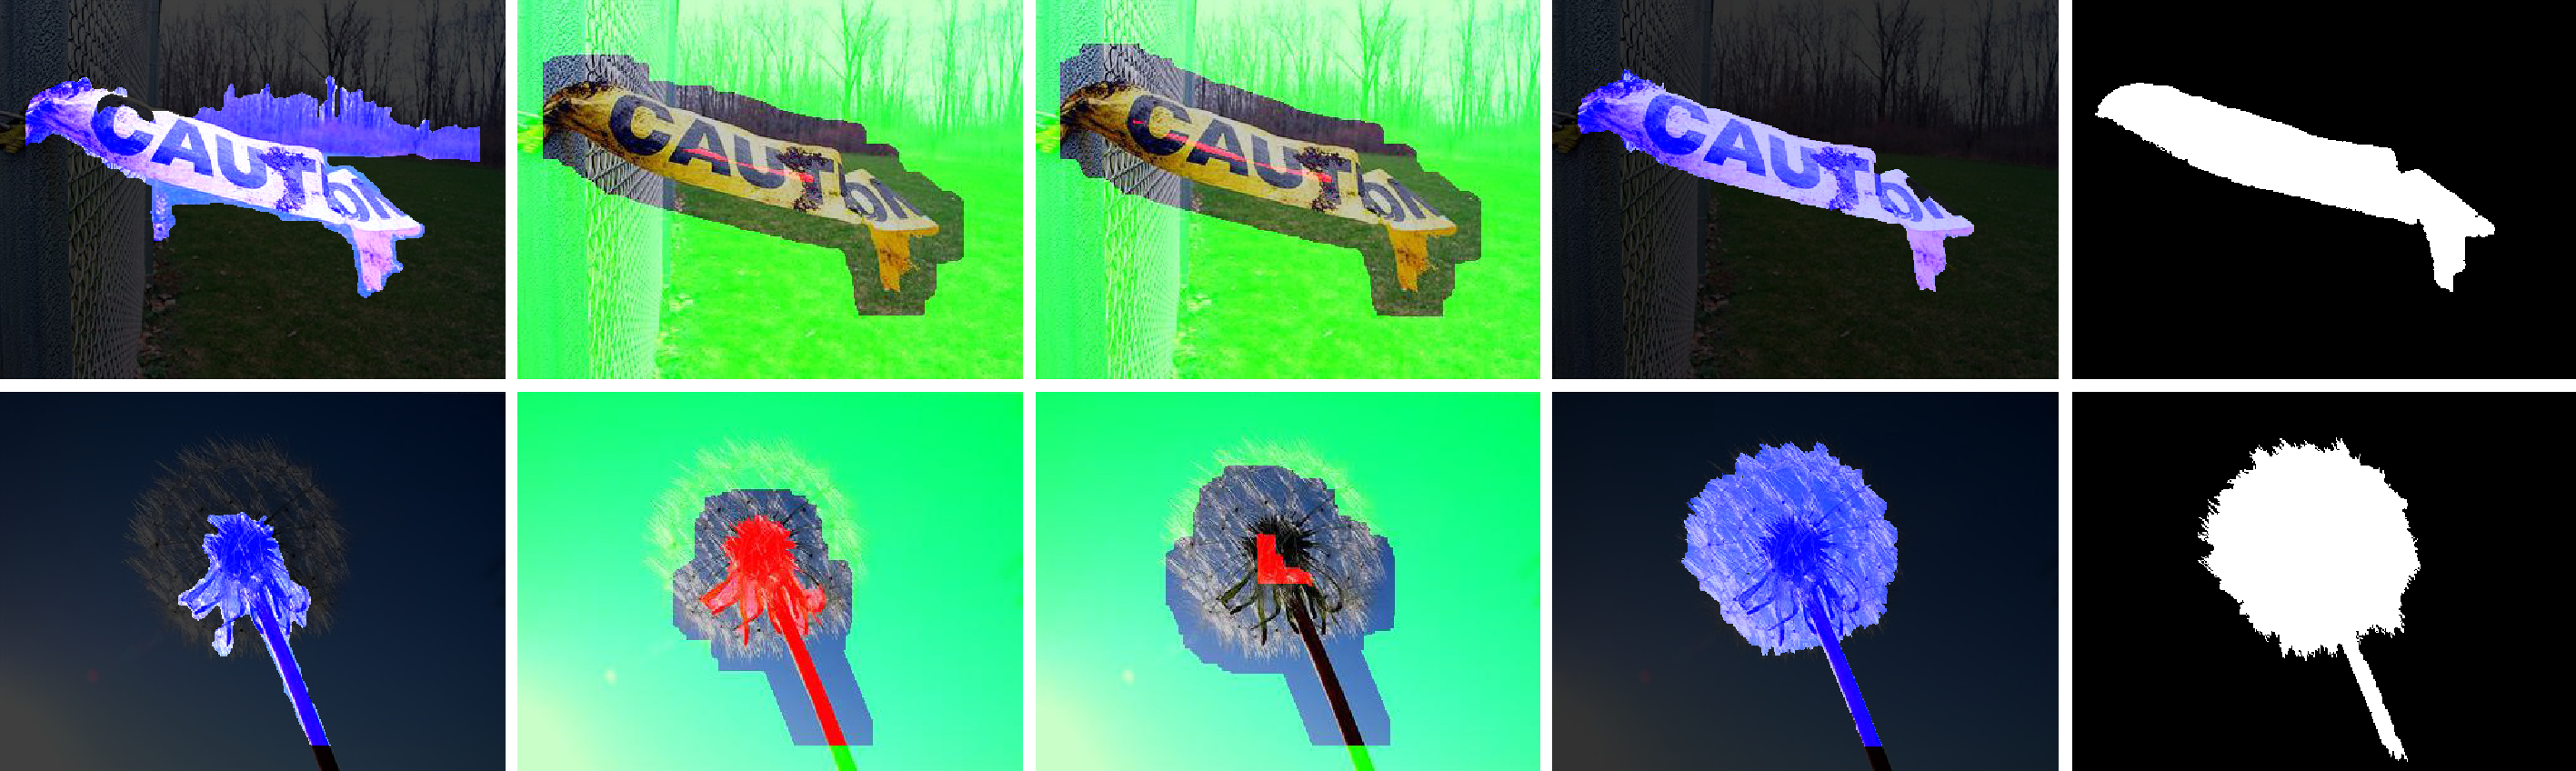
\includegraphics[width=\columnwidth]{saliency_cut.pdf}
    \caption{显著性区域分割。从左到右依次是:初始分割结果、第一次迭代后的trimap,
          第二次迭代后的trimap,最终分割结果,用户标注的基准数据。
          在分割图中,蓝色代表前景,灰色是背景。
          在trimap中,红色是前景,绿色是背景,未知区域为原图颜色。
    }\label{fig:AttCutSteps}
\end{figure}

\begin{figure*}
  \begin{overpic}[width=\linewidth]{cut_compare.pdf}\small
    \put(3,0){(a)~original}
    \put(17,0){(b)~\LC}
    \put(32,0){(c)~\CA}
    \put(46,0){(d)~\FT}
    \put(60,0){(e)~\HC}
    \put(74,0){(f)~\RC}
    \put(87,0){(g)~ground truth}
  \end{overpic}
  \caption{用不同显著性图初始化显著性分割的结果。相应的显著性图在
    \figref{fig:VisualComparison}中.
  }\label{fig:cutCmp}
\end{figure*}

在我们的方法中,我们迭代应用GrabCut \cite{04tog/rother_grabcut} 来改善二值化显著性
图像后得到的分割结果(见\figref{fig:AttCutSteps})。
传统的GrabCut方法是由人工选中矩形区域来进行初始化操作,
而我们用一个固定阈值二值化后的显著性图来得到显著性分割,
并用这个显著性分割来自动地进行GrabCut初始化。
这个阈值的我们经验性的选择固定阈值实验中与$95\%$召回率对应的阈值。


初始化之后,我们迭代运行GrabCut来改进显著性分割结果(在我们的实验中最多迭代 $4$ 次)。
在每一次迭代后,我们用膨胀和腐蚀操作来得到新的Trimap以进行下一次迭代。
如\figref{fig:AttCutSteps}所示,膨胀后仍然落在外面的区域设置成背景,
在腐蚀区域内的设置成前景,其余的区域为Trimap中的未知。
Grubcut本身是用高斯混合模型和Grapcut进行迭代,来改善每一步的区域分割效果,
靠近初始显著性物体区域的部分成为显著性物体的几率更大。
因此,我们的新的初始化方法可以使GrabCut包含显著性区域附近的显著性区域,
并根据颜色特征的差异排除非显著性区域。
在算法实现中,我们设置了狭窄的图像边界区域(15像素宽)作为背景来提高边界区域的收敛速度。


\figref{fig:AttCutSteps}展示了我们显著性分割算法的两个实例。
在旗子的例子中,不需要的区域被正确地排除;
在花朵的例子中,我们的方法扩展了初始显著性区域并收敛得到了精确的分割结果。
为了保持一致性,我们用召回率$95\%$的阈值对显著性图像进行二值化(见\figref{fig:plots})。
我们在基准数据集~\cite{09cvpr/Achanta_FTSaliency}上比较了平均正确率,召回率以及
$F$-测量,其中$F$-测量定义为:
\begin{equation}\label{equ:FMeasure}
    F_{\beta}= \frac{(1+\beta^2)Precision \times
        Recall}{\beta^2 \times Precision + Recall}.
\end{equation}

和Achanta等人\cite{09cvpr/Achanta_FTSaliency}一样,
我们用$\beta^2=0.3$来使正确率的权重高于召回率。
可以从比较结果(见\figref{fig:plots}-右和\figref{fig:cutCmp})中看出,
用我们的 RC 和 HC 显著性图来进行分割明显优于其它方法。
和当今最好的方法相比(正确率=$75\%$, 召回率=$83\%$),我们方法的结果更精确
(正确率=$90\%$, 召回率=$90\%$)。
(我们的演示程序可以从项目主页中得到。)


%%%%%%%%%%%%%%%%%%%%%%%%%%%%%%%%%%%%%%%%%%%%%%%%%%%%
\begin{figure}[t!]
   \begin{overpic}[width=\columnwidth]{contentAware_application.pdf} \small
   \put(3,0){original}
   \put(21,0){CA}
   \put(31,0){RC}
   \put(48,0){original}
   \put(75,0){CA}
   \put(90,0){RC}
    \end{overpic}
    \caption{用\CA 和我们的RC显著性图进行内容敏感的图像缩放
        \cite{09cgf/ZhangC}的结果比较。
    }\label{fig:Resizing}
\end{figure}


\mypara{基于内容感知的图像缩放}
在内容敏感的图像缩放中,显著性图像经常用来指定图像的相对重要区域
(见~\cite{09_image_resize})。
我们用提取出的显著性图像进行了图像缩放实验。
实验中采用了Zhang等人提出的\cite{09cgf/ZhangC}内容敏感图像缩放方法
\footnote{我们采用作者公开的代码}。
该方法通过变形能量将变形分配到相对非显著性区域,同时保持全局和局部的图像特征。
\figref{fig:Resizing}比较了用\RC 和\CA 显著性图像得到的图像缩放结果。
显著性物体区域的显著性值是成片光滑的,这点对于基于能量的缩放非常重要,
因此我们的 RC 显著性图产生更好的缩放结果。
CA显著性图像在物体的边界有更高的显著性值,但这并不适于图像缩放等应用,
这些应用要求整个显著性物体一致的被突出。


%%%%%%%%%%%%%%%%%%%%%%%%%%%%%%%%%%%%%%%%%%%%%%%%%
\mypara{非真实感渲染}
艺术家们经常对图像抽象并突出有意义的部分并掩盖非重要区域\cite{99/zeki_innerVision}。
受此现象启发,一系列用显著性值来进行非真实感渲染的方法产生,
并产生了有趣的结果~\cite{02tog/decarlo_stylization}。
我们将我们的方法和最近的杰出的显著性检测方法~\cite{09cvpr/Achanta_FTSaliency}用在NPR
技术\cite{10pg/Huang_Zhang}上进行了比较(见\figref{fig:NPR})。
我们的\RC 提供更好的掩模,这可以帮助NPR方法更好地保留重要图像部分以及区域边界的细节,
同时平滑其它部分。


%%%%%%%%%%%%%%%%%%%%%%%%%%%%%%%%%%%%%%%%%%%%%%%%%%%%
\begin{figure}[t!]
   \begin{overpic}[width=\columnwidth]{npr_application2.pdf} \small
     \end{overpic}
    \caption{(左,右)~\FT 和RC显著性图分别被用于风格化绘制\cite{10pg/Huang_Zhang}。
        我们的方法生成了更好的显著性图,是的风格化绘制保持了重要部分的细节。例如马头
        和栏杆部分细节更好的保留了。
    }\label{fig:NPR}
\end{figure}


\begin{figure}[t!]
   \begin{overpic}[width=\columnwidth]{challenging_maps.pdf} \small
     \end{overpic}
    \caption{对于我们提出的基于直方图的方法来说一个有挑战性的例子:(上图)显著性区域和
        非显著性区域具有相似的颜色,(下图)图像具有复杂的纹理背景。
        从左到右依次是输入图像、HC显著性图、HC显著性区域分割、RC显著性图、 RC显著性区域分割.
    } \label{fig:challenging_maps}
\end{figure}



%%%%%%%%%%%%%%%%%%%%%%%%%%%%%%%%%%%%%%%%%%%%%%%%%

\section{总结与展望}\label{sec:Conclusion}
我们提出了基于全局对比度的显著性计算方法,即基于直方图对比度~(HC) 和基于空间信息增强的区域对比度~(RC)方法。
HC方法速度快,并且产生细节精确的结果,RC方法可以产生空间增强的高质量显著性图像,但与此同时具有相对较低的计算效率。
我们在国际上现有最大的公开数据集上测试了我们的方法,并与之前已有八种最好的其它方法进行了比较。
实验结果表明,我们提出的方法在正确率和召回率上都明显优于其它方法,并且简单而高效。

在未来的工作中,我们计划研究包含空间关系且保留详细细节的显著性图像的高效计算算法,
并且希望研究能够处理具有复杂纹理的背景图像的显著性检测算法,
以克服我们现有算法在处理这类情况中存在的缺陷。
最后,我们还希望显著性图像的检测过程中进一步考虑人脸、对称性等高级因素。
我们相信显著性图像可以应用于高效物体检测\cite{06TCSVT/han_unsupervised},
可靠图像分类,鲁棒的图像景物分析~\cite{journal/tog/ChengZMHH10},
并提高图像检索效果\cite{tog09/ChenCT_Sketch2Photo}。


\paragraph{致谢.} 本项目受到了国家973计划(2011CB302205), 国家863计划(2009AA01Z327),
国家自然科学基金(U0735001),以及国家核高基计划(2011ZX01042-001-002)的支持.
程明明的工作受到了Google PhD fellowship, IBM PhD fellowship, 以及教育部博士研究生学术新人奖的资助。

{\small
\bibliographystyle{ieee}
\bibliography{Saliency}
}

% \end{CJK*}
\end{document}
